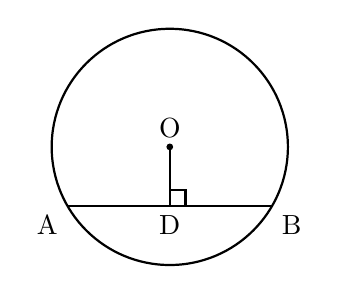
\begin{tikzpicture}[scale=1]

    % Define the center of the circle
    \coordinate (O) at (0,0);

    % Draw the circle
    \draw[thick] (O) circle (1.5);

    % Define points A and B on the circle and D on the chord
    \coordinate (A) at (-1.3, -0.75);
    \coordinate (B) at (1.3, -0.75);
    \coordinate (D) at (0, -0.75);

    % Draw the chord AB
    \draw[thick] (A) -- (B);

    % Draw the line from O to D
    \draw[thick] (O) -- (D);

    % Draw the right-angle symbol at D
    \draw[thick] (0.2, -0.75) -- (0.2, -0.55) -- (0, -0.55);

    % Add a small dot for O
    \filldraw (O) circle (1pt);

    % Add labels for the points
    \node[above] at (O) {O};
    \node[below left] at (A) {A};
    \node[below right] at (B) {B};
    \node[below] at (D) {D};

\end{tikzpicture}